%#######################################################################
%
% Introduction and motivation for open tool support and VDM + UML
%
\section{Tool building in VDM}
%-----------------------------------------------------------------------
%
% Outline
%
\begin{frame}
  \frametitle{Outline}
  \tableofcontents[current]
\end{frame}



%
% Improce Tools support
%
\frame
{
  \frametitle{Tool building in VDM}
\begin{center}
  \begin{itemize}
	%\itemsep=1cm
  		\item AST creation in VDM-SL
  		\item VDM for modling of AST
  		\item VDM Tools code generator to Java
  		\item Eclipse plug-in building.
	  	
  \end{itemize}

\end{center}
}







%-----------------------------------------------------------------------
\subsection{AST modeling}
%-----------------------------------------------------------------------

%
% UML Transformation overview
%
\frame
{
  \frametitle{AST creation}

\begin{center}
\begin{figure}
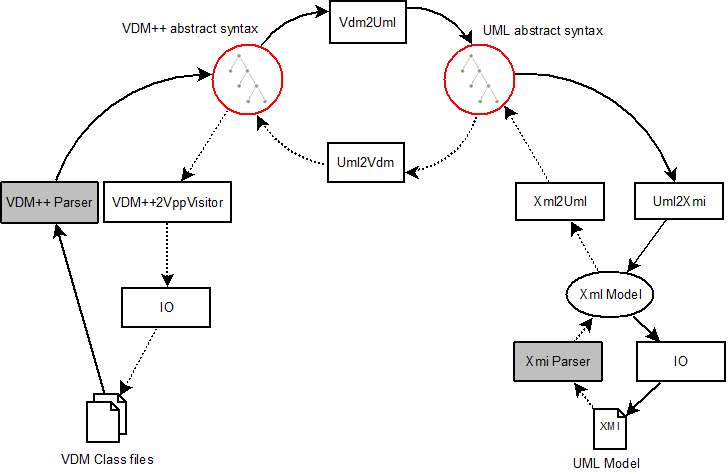
\includegraphics[width=\textwidth]{images/OverviewOverMappingAST.png}
\end{figure}
\end{center}
}


%
% Overview of supported features
%
\frame
{
  \frametitle{Creating AST's from VDM-SL}
\begin{center}



\begin{columns}
\begin{column}[l]{4cm}

  \begin{itemize}
	%\itemsep=1cm
  		\item Create VDM-SL tree
  		\item ASTGen to VDM and Java
  		\item Model in VDM
  		\item VDM Tools code generator to Java
  \end{itemize}

\end{column}
\begin{column}[r]{6cm}

\vdmSpecLineNum{UMLAST_Class.ast}{}{VDM:Collections}


\end{column}
\end{columns}


\end{center}
}


%-----------------------------------------------------------------------
\subsection{Transformation modeling}
%-----------------------------------------------------------------------

%
% Overview Modeling
%
\frame
{
  \frametitle{VDM model}
\begin{center}


\vdmSpecLineNum{Vdm2UmlBuild_class.vpp}{}{VDM:Collections}



\end{center}
}

%-----------------------------------------------------------------------
\subsection{Code generating}
%-----------------------------------------------------------------------


%
% UML Transformation overview
%
\frame
{
  \frametitle{Code generation overview}

\begin{center}

\begin{figure}

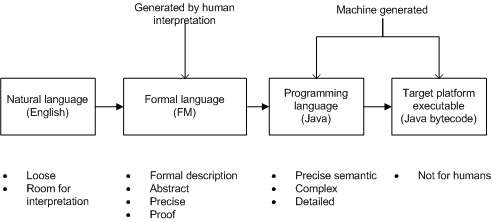
\includegraphics[width=\textwidth]{images/codegenneration.png}

\end{figure}

\end{center}
}
